\chapter{Circuit management}

\section{CREATE and CREATED cells}
Users set up circuits incrementally, one hop at a time. To create a
new circuit, OPs send a CREATE/CREATE2 cell to the first node, with
the first half of an authenticated handshake; that node responds with
a CREATED/CREATED2 cell with the second half of the handshake. To
extend a circuit past the first hop, the OP sends an EXTEND/EXTEND2
relay cell, which instructs the last node in the
circuit to send a CREATE/CREATE2 cell to extend the circuit.

\paragraph{}
There are two kinds of CREATE and CREATED cells: The older
"CREATE/CREATED" format, and the newer "CREATE2/CREATED2" format. The
newer format is extensible by design; the older one is not.

\paragraph{}
A CREATE2 cell contains:

\begin{verbatim}
    HTYPE (Client Handshake Type) [2 bytes]
    HLEN (Client Handshake Data Len) [2 bytes]
    HDATA (Client Handshake Data) [HLEN bytes]
\end{verbatim}

\paragraph{}
A CREATED2 cell contains:

\begin{verbatim}
    HLEN (Server Handshake Data Len) [2 bytes]
    HDATA (Server Handshake Data) [HLEN bytes]
\end{verbatim}

\paragraph{}
Recognized handshake types are:

\begin{verbatim}
    0x0000 TAP -- the original Tor handshake
    0x0001 reserved
    0x0002 ntor -- the ntor+curve25519+sha256 handshake
\end{verbatim}

\paragraph{}
The format of a CREATE cell is one of the following:

\begin{verbatim}
    HDATA (Client Handshake Data) [TAP_C_HANDSHAKE_LEN bytes]
\end{verbatim}
\paragraph{}
or
\begin{verbatim}
    HTAG (Client Handshake Type Tag) [16 bytes]
    HDATA (Client Handshake Data) [TAP_C_HANDSHAKE_LEN-16 bytes]
\end{verbatim}

\paragraph{}
The first format is equivalent to a CREATE2 cell with HTYPE of 'tap'
and length of TAP\_C\_HANDSHAKE\_LEN. The second format is a way to
encapsulate new handshake types into the old CREATE cell format for
migration. Recognized HTAG values are:

\begin{verbatim}
    ntor -- 'ntorNTORntorNTOR'
\end{verbatim}

\paragraph{}
The format of a CREATED cell is:

\begin{verbatim}
    HDATA (Server Handshake Data) [TAP_S_HANDSHAKE_LEN bytes]
\end{verbatim}

\paragraph{}
(It's equivalent to a CREATED2 cell with length of TAP\_S\_HANDSHAKE\_LEN.)

\paragraph{}
As usual with DH, x and y MUST be generated randomly.

\paragraph{}
In general, clients SHOULD use CREATE whenever they are using the TAP
handshake, and CREATE2 otherwise. Clients SHOULD NOT send the
second format of CREATE cells (the one with the handshake type tag)
to a server directly.

\paragraph{}
Servers always reply to a successful CREATE with a CREATED, and to a
successful CREATE2 with a CREATED2. On failure, a server sends a
DESTROY cell to tear down the circuit.

\paragraph{}
[CREATE2 is handled by Tor 0.2.4.7-alpha and later.]

\subsection{Handling CREATED Cells}

When CREATED/CREATED2 cells are parsed and checked, they are handed off to a
CPUWorker as a task. If the queue is full, tasks will be added to the pending
queue. Otherwise, a cpuworker\_request\_t will be build with the received handshake
data. A cpuworker\_job\_t will then be created containing the cpuworker request.

\paragraph{}
The job will further be encapsulated in a workqueue\_entry\_t instance and will be
added to queue of entries. Whenever a thread becomes idle, it will dequeue this entry
and call on the request the cpuworker\_onion\_handshake\_threadfn function, which will
generate the handshake answer based on the on its type, and will save it in the
cpuworker\_reply\_t field of the job. The reply will be added to reply\_queue.
Reply's type will be CREATED/CREATED2/CREATED\_FAST.

\paragraph{}
the cpuworker\_onion\_handshake\_replyfn function will later be called upon the reply, which
will append the CREATED cell to the circuit queue, to be sent on the network to the
initiating node.


\subsection{Choosing circuit IDs in create cells}
The CircID for a CREATE/CREATE2 cell is an arbitrarily chosen
nonzero integer, selected by the node (OP or OR) that sends the
CREATE/CREATE2 cell. In link protocol 3 or lower, CircIDs are 2
bytes long; in protocol 4 or higher, CircIDs are 4 bytes long.

\paragraph{}
To prevent CircID collisions, when one node sends a CREATE/CREATE2
cell to another, it chooses from only one half of the possible
values based on the ORs' public identity keys.

\paragraph{}
In link protocol version 3 or lower, if the sending node has a lower
key, it chooses a CircID with an MSB of 0; otherwise, it chooses a
CircID with an MSB of 1. (Public keys are compared numerically by
modulus.) With protocol version 3 or lower, a client with no public key
MAY choose any CircID it wishes, since clients never need to process a
CREATE/CREATE2 cell.

\paragraph{}
In link protocol version 4 or higher, whichever node initiated the
connection sets its MSB to 1, and whichever node didn't initiate the
connection sets its MSB to 0.

\paragraph{}
The CircID value 0 is specifically reserved for cells that do not
belong to any circuit: CircID 0 must not be used for circuits. No
other CircID value, including 0x8000 or 0x80000000, is reserved.

\subsection{EXTEND and EXTENDED cells}
To extend an existing circuit, the client sends an EXTEND or EXTEND2
relay cell to the last node in the circuit.
An EXTEND2 cell's relay payload contains:

\begin{verbatim}
    NSPEC (Number of link specifiers) [1 byte]
    NSPEC times:
        LSTYPE (Link specifier type) [1 byte]
        LSLEN (Link specifier length) [1 byte]
        LSPEC (Link specifier) [LSLEN bytes]
    HTYPE (Client Handshake Type) [2 bytes]
    HLEN (Client Handshake Data Len) [2 bytes]
    HDATA (Client Handshake Data) [HLEN bytes]
\end{verbatim}

Link specifiers describe the next node in the circuit and how to
connect to it. Recognized specifiers are:
\begin{itemize}
    \item [00] TLS-over-TCP, IPv4 address
    A four-byte IPv4 address plus two-byte ORPort
    \item [01] TLS-over-TCP, IPv6 address
    A sixteen-byte IPv6 address plus two-byte ORPort
    \item [02] Legacy identity
    A 20-byte SHA1 identity fingerprint. At most one may be listed.
    \item [03] Ed25519 identity
    A 32-byte Ed25519 identity fingerprint. At most one may
    be listed.
\end{itemize}

\paragraph{}
Nodes MUST ignore unrecognized specifiers, and MUST accept multiple
instances of specifiers other than 'legacy identity'.

\paragraph{}
The relay payload for an EXTEND relay cell consists of:
\begin{verbatim}
    Address [4 bytes]
    Port [2 bytes]
    Onion skin [TAP_C_HANDSHAKE_LEN bytes]
    Identity fingerprint [HASH_LEN bytes]
\end{verbatim}

\paragraph{}
The "legacy identity" and "identity fingerprint" fields are the
SHA1 hash of the PKCS\#1 ASN1 encoding of the next onion router's
identity (signing) key. (See 0.3 above.) The "Ed25519 identity"
field is the Ed25519 identity key of the target node. Including
this key information allows the extending OR verify that it is
indeed connected to the correct target OR, and prevents certain
man-in-the-middle attacks.

\paragraph{}
Extending ORs MUST check \textit{all} provided identity keys (if they
recognize the format), and MUST NOT extend the circuit if the
target OR did not prove its ownership of any such identity key.
If only one identity key is provided, but the extending OR knows
the other (from directory information), then the OR SHOULD also
enforce that key.

\paragraph{}
If an extending OR has a channel with a given Ed25519 ID and RSA
identity, and receives a request for that Ed25519 ID and a
different RSA identity, it SHOULD NOT attempt to make another
connection: it should just fail and DESTROY the circuit.
After checking relay identities, extending ORs generate a
CREATE/CREATE2 cell from the contents of the EXTEND/EXTEND2 cell.

\paragraph{}
The payload of an EXTENDED cell is the same as the payload of a
CREATED cell.

\paragraph{}
The payload of an EXTENDED2 cell is the same as the payload of a
CREATED2 cell.

\paragraph{}
[Support for EXTEND2/EXTENDED2 was added in Tor 0.2.4.8-alpha.]

\paragraph{}
Clients SHOULD use the EXTEND format whenever sending a TAP
handshake, and MUST use it whenever the EXTEND cell will be handled
by a node running a version of Tor too old to support EXTEND2. In
other cases, clients SHOULD use EXTEND2.

\paragraph{}
When generating an EXTEND2 cell, clients SHOULD include the target's
Ed25519 identity whenever the target has one, and whenever the
target supports LinkAuth subprotocol version "3".

\paragraph{}
When encoding a non-TAP handshake in an EXTEND cell, clients SHOULD
use the format with 'client handshake type tag'.

\subsection{The "TAP" handshake}
This handshake uses Diffie-Hellman in Z\_p and RSA to compute a set of
shared keys which the client knows are shared only with a particular
server, and the server knows are shared with whomever sent the
original handshake (or with nobody at all). It's not very fast and
not very good. (See Goldberg's "On the Security of the Tor
Authentication Protocol".)

\begin{verbatim}
    Define TAP_C_HANDSHAKE_LEN as DH_LEN+KEY_LEN+PK_PAD_LEN.
    Define TAP_S_HANDSHAKE_LEN as DH_LEN+HASH_LEN.
\end{verbatim}

\paragraph{}
The payload for a CREATE cell is an 'onion skin', which consists of
the first step of the DH handshake data (also known as $g^x$). This
value is encrypted using the "legacy hybrid encryption" algorithm
(see 0.4 above) to the server's onion key, giving a client handshake:

\begin{verbatim}
    PK-encrypted:
        Padding [PK_PAD_LEN bytes]
        Symmetric key [KEY_LEN bytes]
        First part of g^x [PK_ENC_LEN-PK_PAD_LEN-KEY_LEN bytes]
    Symmetrically encrypted:
        Second part of g^x [DH_LEN-(PK_ENC_LEN-PK_PAD_LEN-KEY_LEN) bytes]
\end{verbatim}

\paragraph{}
The payload for a CREATED cell, or the relay payload for an
EXTENDED cell, contains:

\begin{verbatim}
    DH data (g^y) [DH_LEN bytes]
    Derivative key data (KH) [HASH_LEN bytes]
\end{verbatim}

\paragraph{}
Once the handshake between the OP and an OR is completed, both can
now calculate $g^{xy}$ with ordinary DH. Before computing $g^{xy}$, both parties
MUST verify that the received $g^x$ or $g^y$ value is not degenerate;
that is, it must be strictly greater than 1 and strictly less than p-1
where p is the DH modulus. Implementations MUST NOT complete a handshake
with degenerate keys. Implementations MUST NOT discard other "weak"
$g^x$ values.

\paragraph{}
(Discarding degenerate keys is critical for security; if bad keys
are not discarded, an attacker can substitute the OR's CREATED
cell's $g^y$ with 0 or 1, thus creating a known $g^{xy}$ and impersonating
the OR. Discarding other keys may allow attacks to learn bits of
the private key.)

\paragraph{}
Once both parties have $g^{xy}$, they derive their shared circuit keys
and 'derivative key data' value via the KDF-TOR function.

\subsection{The "ntor" handshake}
This handshake uses a set of DH handshakes to compute a set of
shared keys which the client knows are shared only with a particular
server, and the server knows are shared with whomever sent the
original handshake (or with nobody at all). Here we use the
"curve25519" group and representation as specified in "Curve25519:
new Diffie-Hellman speed records" by D. J. Bernstein.

\paragraph{}
[The ntor handshake was added in Tor 0.2.4.8-alpha.]

\paragraph{}
In this section, define:

\begin{verbatim}
    H(x,t) as HMAC_SHA256 with message x and key t.
    H_LENGTH = 32.
    ID_LENGTH = 20.
    G_LENGTH = 32
    PROTOID = "ntor-curve25519-sha256-1"
    t_mac = PROTOID | ":mac"
    t_key = PROTOID | ":key_extract"
    t_verify = PROTOID | ":verify"
    MULT(a,b) = the multiplication of the curve25519 point 'a' by the
                scalar 'b'.
    G = The preferred base point for curve25519 ([9])
    KEYGEN() = The curve25519 key generation algorithm, returning a
               private/public keypair.
    m_expand = PROTOID | ":key_expand"
    KEYID(A) = A
\end{verbatim}

\paragraph{}
To perform the handshake, the client needs to know an identity key
digest for the server, and an ntor onion key (a curve25519 public
key) for that server. Call the ntor onion key "B". The client
generates a temporary keypair:

\begin{verbatim}
    x,X = KEYGEN()
\end{verbatim}

\paragraph{}
and generates a client-side handshake with contents:
\begin{verbatim}
    NODEID Server identity digest [ID_LENGTH bytes]
    KEYID KEYID(B) [H_LENGTH bytes]
    CLIENT_PK X [G_LENGTH bytes]
\end{verbatim}

\paragraph{}
The server generates a keypair of y,Y = KEYGEN(), and uses its ntor
private key 'b' to compute:

\begin{verbatim}
    secret_input = EXP(X,y) | EXP(X,b) | ID | B | X | Y | PROTOID
    KEY_SEED = H(secret_input, t_key)
    verify = H(secret_input, t_verify)
    auth_input = verify | ID | B | Y | X | PROTOID | "Server"
\end{verbatim}

\paragraph{}
The server's handshake reply is:

\begin{verbatim}
    SERVER_PK Y [G_LENGTH bytes]
    AUTH H(auth_input, t_mac) [H_LENGTH bytes]
\end{verbatim}

\paragraph{}
The client then checks Y is in $G^*$ [see NOTE below], and computes

\begin{verbatim}
    secret_input = EXP(Y,x) | EXP(B,x) | ID | B | X | Y | PROTOID
    KEY_SEED = H(secret_input, t_key)
    verify = H(secret_input, t_verify)
    auth_input = verify | ID | B | Y | X | PROTOID | "Server"
\end{verbatim}

\paragraph{}
The client verifies that AUTH == H(auth\_input, t\_mac).

\paragraph{}
Both parties check that none of the EXP() operations produced the
point at infinity. [NOTE: This is an adequate replacement for
checking Y for group membership, if the group is curve25519.]

\paragraph{}
Both parties now have a shared value for KEY\_SEED. They expand this
into the keys needed for the Tor relay protocol, using the KDF
 and the tag m\_expand.

\subsection{CREATE\_FAST/CREATED\_FAST cells}
When initializing the first hop of a circuit, the OP has already
established the OR's identity and negotiated a secret key using TLS.
Because of this, it is not always necessary for the OP to perform the
public key operations to create a circuit. In this case, the
OP MAY send a CREATE\_FAST cell instead of a CREATE cell for the first
hop only. The OR responds with a CREATED\_FAST cell, and the circuit is
created.

\paragraph{}
A CREATE\_FAST cell contains:

\begin{verbatim}
    Key material (X) [HASH_LEN bytes]
\end{verbatim}

\paragraph{}
A CREATED\_FAST cell contains:

\begin{verbatim}
    Key material (Y) [HASH_LEN bytes]
    Derivative key data [HASH_LEN bytes]
\end{verbatim}

\paragraph{}
The values of X and Y must be generated randomly.

\paragraph{}
Once both parties have X and Y, they derive their shared circuit keys
and 'derivative key data' value via the KDF-TOR function.

\paragraph{}
The CREATE\_FAST handshake is currently deprecated whenever it is not
necessary;

\paragraph{}
[Tor 0.3.1.1-alpha and later disable CREATE\_FAST by default.]

\section{Setting circuit keys}

\subsection{KDF-TOR}
This key derivation function is used by the TAP and CREATE\_FAST
handshakes, and in the current hidden service protocol. It shouldn't
be used for new functionality.

\paragraph{}
If the TAP handshake is used to extend a circuit, both parties
base their key material on K0=$g^{xy}$, represented as a big-endian unsigned
integer.

\paragraph{}
If CREATE\_FAST is used, both parties base their key material on
K0=X|Y.

\paragraph{}
From the base key material K0, they compute KEY\_LEN*2+HASH\_LEN*3 bytes of
derivative key data as
\begin{verbatim}
    K = H(K0 | [00]) | H(K0 | [01]) | H(K0 | [02]) | ...
\end{verbatim}

\paragraph{}

The first HASH\_LEN bytes of K form KH; the next HASH\_LEN form the forward
digest Df; the next HASH\_LEN 41-60 form the backward digest Db; the next
KEY\_LEN 61-76 form Kf, and the final KEY\_LEN form Kb. Excess bytes from K
are discarded.

\paragraph{}
\begin{itemize}
    \item KH is used in the handshake response to demonstrate knowledge of the
    computed shared key;
    \item Df is used to seed the integrity-checking hash
    for the stream of data going from the OP to the OR;
    \item Db seeds the integrity-checking hash for the data stream from the OR to the OP;
    \item Kf is used to encrypt the stream of data going from the OP to the OR;
    \item Kb is used to encrypt the stream of data going from the OR to the OP.
\end{itemize}

\subsection{KDF-RFC5869}
For newer KDF needs, Tor uses the key derivation function HKDF from
RFC5869, instantiated with SHA256. (This is due to a construction
from Krawczyk.) The generated key material is:

\begin{verbatim}
    K = K_1 | K_2 | K_3 | ...
\end{verbatim}

\paragraph{}
Where

\begin{itemize}
    \item H(x,t) is HMAC\_SHA256 with value x and key t
    \item K\_1 = H(m\_expand | INT8(1) , KEY\_SEED )
    \item K\_(i+1) = H(K\_i | m\_expand | INT8(i+1) , KEY\_SEED )
    \item m\_expand is an arbitrarily chosen value,
    \item INT8(i) is a octet with the value "i".
\end{itemize}

\paragraph{}
In RFC5869's vocabulary, this is HKDF-SHA256 with

\begin{verbatim}
    info == m_expand,
    salt == t_key,
    IKM == secret_input.
\end{verbatim}

\paragraph{}
When used in the ntor handshake, the first HASH\_LEN bytes form the
forward digest Df; the next HASH\_LEN form the backward digest Db; the
next KEY\_LEN form Kf, the next KEY\_LEN form Kb, and the final
DIGEST\_LEN bytes are taken as a nonce to use in the place of KH in the
hidden service protocol. Excess bytes from K are discarded.

\section{Creating circuits}

When creating a circuit through the network, the circuit creator
(OP) performs the following steps:

\begin{enumerate}
    \item Choose an onion router as an end node (R\_N)
    \begin{itemize}
        \item N MAY be 1 for non-anonymous directory mirror, introduction point,
        or service rendezvous connections.
        \item N SHOULD be 3 or more for anonymous connections \ref{fig:circuit_tor} .
        Some end nodes accept streams, others are introduction
        or rendezvous points (see rend-spec-{v2,v3}.txt).
        \begin{figure}[h]
			\centering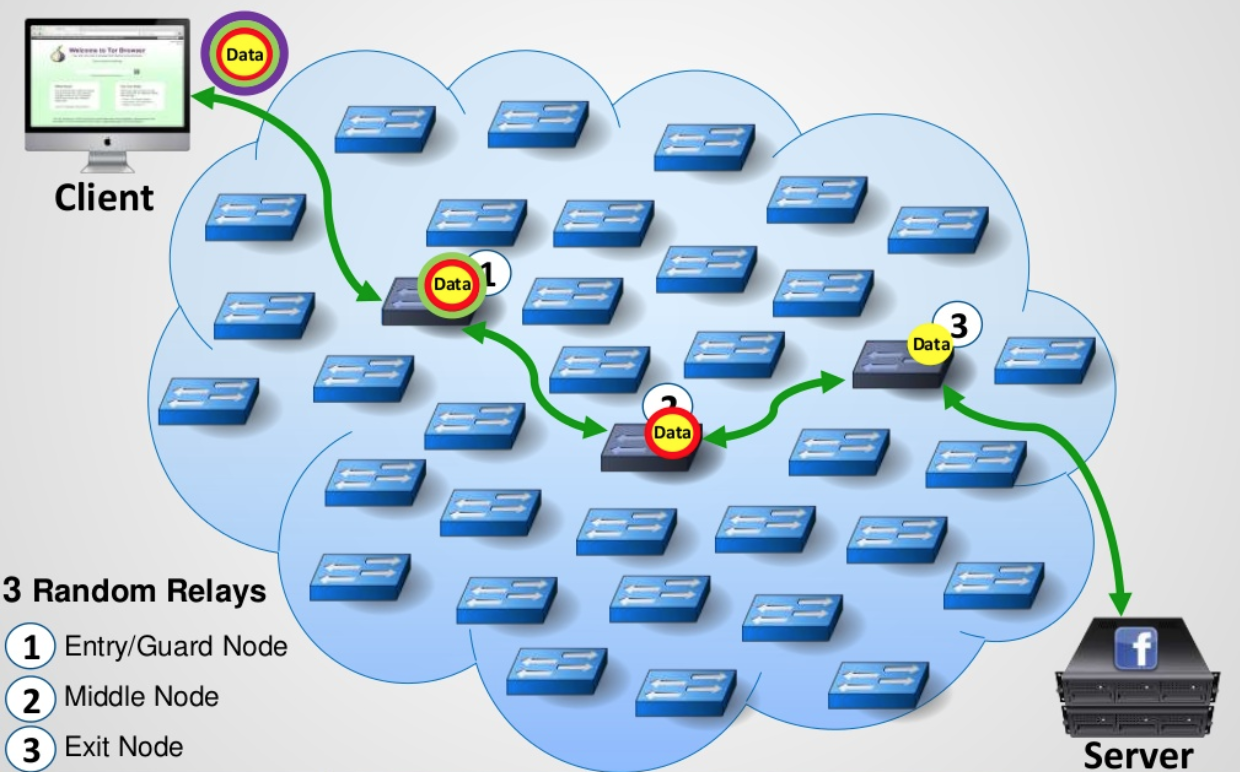
\includegraphics[scale=0.35]{circuit_tor}
			\caption{Tor Circuit Creation \cite{tor_slideshare}}
			\label{fig:circuit_tor} % Unique label used for referencing the figure in-text
			\end{figure}
    \end{itemize}
    \item Choose a chain of (N-1) onion routers (R\_1...R\_N-1) to constitute
    the path, such that no router appears in the path twice.

    \item If not already connected to the first router in the chain,
    open a new connection to that router.

    \item Choose a circID not already in use on the connection with the
    first router in the chain; send a CREATE/CREATE2 cell along
    the connection, to be received by the first onion router.

    \item Wait until a CREATED/CREATED2 cell is received; finish the
    handshake and extract the forward key Kf\_1 and the backward
    key Kb\_1.

    \item For each subsequent onion router R (R\_2 through R\_N), extend
    the circuit to R.
\end{enumerate}

To extend the circuit by a single onion router R\_M, the OP performs
these steps:
\begin{enumerate}
    \item Create an onion skin, encrypted to R\_M's public onion key.

    \item Send the onion skin in a relay EXTEND/EXTEND2 cell along
    the circuit (see sections 5.1.2 and 5.5).

    \item When a relay EXTENDED/EXTENDED2 cell is received, verify KH,
    and calculate the shared keys. The circuit is now extended.
    When an onion router receives an EXTEND relay cell, it sends a CREATE
    cell to the next onion router, with the enclosed onion skin as its
    payload.
\end{enumerate}

\paragraph{}
When an onion router receives an EXTEND2 relay cell, it sends a CREATE2
cell to the next onion router, with the enclosed HLEN, HTYPE, and HDATA
as its payload.

\paragraph{}
As special cases, if the EXTEND/EXTEND2 cell includes a legacy
identity, identity fingerprint, or Ed25519 identity of all zeroes, or
asks to extend back to the relay that sent the extend cell, the
circuit will fail and be torn down. The initiating onion router
chooses some circID not yet used on the connection between the two
onion routers.

\paragraph{}
When an onion router receives a CREATE/CREATE2 cell, if it already has a
circuit on the given connection with the given circID, it drops the
cell. Otherwise, after receiving the CREATE/CREATE2 cell, it completes
the specified handshake, and replies with a CREATED/CREATED2 cell.

\paragraph{}
Upon receiving a CREATED/CREATED2 cell, an onion router packs it payload
into an EXTENDED/EXTENDED2 relay cell, and sends
that cell up the circuit. Upon receiving the EXTENDED/EXTENDED2 relay
cell, the OP can retrieve the handshake material.

\paragraph{}
(As an optimization, OR implementations may delay processing onions
until a break in traffic allows time to do so without harming
network latency too greatly.)


\subsection{Canonical connections}
It is possible for an attacker to launch a man-in-the-middle attack
against a connection by telling OR Alice to extend to OR Bob at some
address X controlled by the attacker. The attacker cannot read the
encrypted traffic, but the attacker is now in a position to count all
bytes sent between Alice and Bob (assuming Alice was not already
connected to Bob.)

\paragraph{}
To prevent this, when an OR gets an extend request, it SHOULD use an
existing OR connection if the ID matches, and ANY of the following
conditions hold:

\begin{itemize}
    \item The IP matches the requested IP.
    \item The OR knows that the IP of the connection it's using is canonical
    because it was listed in the NETINFO cell.
    \item The OR knows that the IP of the connection it's using is canonical
    because it was listed in the server descriptor.
\end{itemize}

\section{Tearing down circuits}
Circuits are torn down when an unrecoverable error occurs along
the circuit, or when all streams on a circuit are closed and the
circuit's intended lifetime is over.

\paragraph{}
ORs SHOULD also tear down circuits which attempt to create:

\begin{itemize}
    \item streams with RELAY\_BEGIN, or
    \item rendezvous points with ESTABLISH\_RENDEZVOUS;
\end{itemize}

\paragraph{}
ending at the first hop. Letting Tor be used as a single hop proxy makes
exit and rendezvous nodes a more attractive target for compromise.

\paragraph{}
ORs MAY use multiple methods to check if they are the first hop:

\begin{itemize}
    \item If an OR sees a circuit created with CREATE\_FAST, the OR is sure to be
    the first hop of a circuit.
    \item If an OR is the responder, and the initiator:
    \begin{itemize}
        \item did not authenticate the link, or
        \item authenticated with a key that is not in the consensus,
        then the OR is probably the first hop of a circuit (or the second hop of
        a circuit via a bridge relay).
    \end{itemize}
\end{itemize}

\paragraph{}
Circuits may be torn down either completely or hop-by-hop.

\paragraph{}
To tear down a circuit completely, an OR or OP sends a DESTROY
cell to the adjacent nodes on that circuit, using the appropriate
direction's circID.

\paragraph{}
Upon receiving an outgoing DESTROY cell, an OR frees resources
associated with the corresponding circuit. If it's not the end of
the circuit, it sends a DESTROY cell for that circuit to the next OR
in the circuit. If the node is the end of the circuit, then it tears
down any associated edge connections.

\paragraph{}
After a DESTROY cell has been processed, an OR ignores all data or
destroy cells for the corresponding circuit.

\paragraph{}
To tear down part of a circuit, the OP may send a RELAY\_TRUNCATE cell
signaling a given OR (Stream ID zero). That OR sends a DESTROY
cell to the next node in the circuit, and replies to the OP with a
RELAY\_TRUNCATED cell.

\paragraph{}
[Note: If an OR receives a TRUNCATE cell and it has any RELAY cells
still queued on the circuit for the next node it will drop them
without sending them. This is not considered conformant behavior,
but it probably won't get fixed until a later version of Tor. Thus,
clients SHOULD NOT send a TRUNCATE cell to a node running any current
version of Tor if a) they have sent relay cells through that node,
and b) they aren't sure whether those cells have been sent on yet.]

\paragraph{}
When an unrecoverable error occurs along one connection in a
circuit, the nodes on either side of the connection should, if they
are able, act as follows: the node closer to the OP should send a
RELAY\_TRUNCATED cell towards the OP; the node farther from the OP
should send a DESTROY cell down the circuit.

\paragraph{}
The payload of a RELAY\_TRUNCATED or DESTROY cell contains a single octet,
describing why the circuit is being closed or truncated. When sending a
TRUNCATED or DESTROY cell because of another TRUNCATED or DESTROY cell,
the error code should be propagated. The origin of a circuit always sets
this error code to 0, to avoid leaking its version. The error codes are:

\begin{enumerate}
    \item NONE (No reason given.)
    \item PROTOCOL (Tor protocol violation.)
    \item INTERNAL (Internal error.)
    \item REQUESTED (A client sent a TRUNCATE command.)
    \item HIBERNATING (Not currently operating; trying to save bandwidth.)
    \item RESOURCELIMIT (Out of memory, sockets, or circuit IDs.)
    \item CONNECTFAILED (Unable to reach relay.)
    \item OR\_IDENTITY (Connected to relay, but its OR identity was not
    as expected.)
    \item OR\_CONN\_CLOSED (The OR connection that was carrying this circuit
    died.)
    \item FINISHED (The circuit has expired for being dirty or old.)
    \item TIMEOUT (Circuit construction took too long)
    \item DESTROYED (The circuit was destroyed w/o client TRUNCATE)
    \item NOSUCHSERVICE (Request for unknown hidden service)
\end{enumerate}

\section{Routing relay cells}

\subsection{Circuit ID Checks}

When a node wants to send a RELAY or RELAY\_EARLY cell, it checks the cell's
circID and determines whether the corresponding circuit along that
connection is still open. If not, the node drops the cell.

\paragraph{}
When a node receives a RELAY or RELAY\_EARLY cell, it checks the cell's
circID and determines whether it has a corresponding circuit along
that connection. If not, the node drops the cell.

\subsection{Forward Direction}
The forward direction is the direction that CREATE/CREATE2 cells
are sent.

\subsubsection{Routing from the Origin}
When a relay cell is sent from an OP, the OP encrypts the payload
with the stream cipher as follows:

\begin{verbatim}
    OP sends relay cell:
        For I=N...1, where N is the destination node:
            Encrypt with Kf_I.
        Transmit the encrypted cell to node 1.
\end{verbatim}


\subsubsection{Relaying Forward at Onion Routers}
When a forward relay cell is received by an OR, it decrypts the payload
with the stream cipher, as follows:
\begin{verbatim}
    'Forward' relay cell:
        Use Kf as key; decrypt.
\end{verbatim}

\paragraph{}
The OR then decides whether it recognizes the relay cell, by
inspecting the payload. If the OR
recognizes the cell, it processes the contents of the relay cell.
Otherwise, it passes the decrypted relay cell along the circuit if
the circuit continues. If the OR at the end of the circuit
encounters an unrecognized relay cell, an error has occurred: the OR
sends a DESTROY cell to tear down the circuit.

\paragraph{}
For more information, see section 6 below.

\subsection{Backward Direction}
The backward direction is the opposite direction from
CREATE/CREATE2 cells.

\subsubsection{Relaying Backward at Onion Routers}
When a backward relay cell is received by an OR, it encrypts the payload
with the stream cipher, as follows:
\begin{verbatim}
    'Backward' relay cell:
        Use Kb as key; encrypt.
\end{verbatim}

\subsubsection{Routing to the Origin}
When a relay cell arrives at an OP, the OP decrypts the payload
with the stream cipher as follows:
\begin{verbatim}
    OP receives relay cell from node 1:
        For I=1...N, where N is the final node on the circuit:
\end{verbatim}

\subsection{Handling relay\_early cells}
A RELAY\_EARLY cell is designed to limit the length any circuit can reach.
When an OR receives a RELAY\_EARLY cell, and the next node in the circuit
is speaking v2 of the link protocol or later, the OR relays the cell as a
RELAY\_EARLY cell. Otherwise, older Tors will relay it as a RELAY cell.

\paragraph{}
If a node ever receives more than 8 RELAY\_EARLY cells on a given
outbound circuit, it SHOULD close the circuit. If it receives any
inbound RELAY\_EARLY cells, it MUST close the circuit immediately.

\paragraph{}
When speaking v2 of the link protocol or later, clients MUST only send
EXTEND/EXTEND2 cells inside RELAY\_EARLY cells. Clients SHOULD send the first ~8
RELAY cells that are not targeted at the first hop of any circuit as
RELAY\_EARLY cells too, in order to partially conceal the circuit length.

\paragraph{}
[Starting with Tor 0.2.3.11-alpha, relays should reject any
EXTEND/EXTEND2 cell not received in a RELAY\_EARLY cell.]